% Provenance (never printed): cycle 3 / 6e "La planete Terre" (rocks and
% minerals; the three rock families; recognising common rocks); see
% sources/book1/PROVENANCE.md. Book 1, grade 6, chapter 3.
% Vocabulary guard: "magma" not before g7.2 (here "molten rock");
% "sediment" not before g7.4 (here "grains of sand and mud").
\chapter{Rocas y minerales}\label{ch:g6:rocks-and-minerals}

Sam se inclina sobre la encimera de la cocina con una lupa. La piedra
pulida, que de lejos parece gris, se convierte en una multitud de motas:
unas rosas, otras blancas, otras grises y vidriosas, y otras negras y
diminutas que brillan cuando les da la luz. Cada mota tiene caras planas y
brillantes, y las motas encajan entre sí como las piezas de un
rompecabezas. ¿Qué son?

\begin{omfigure}
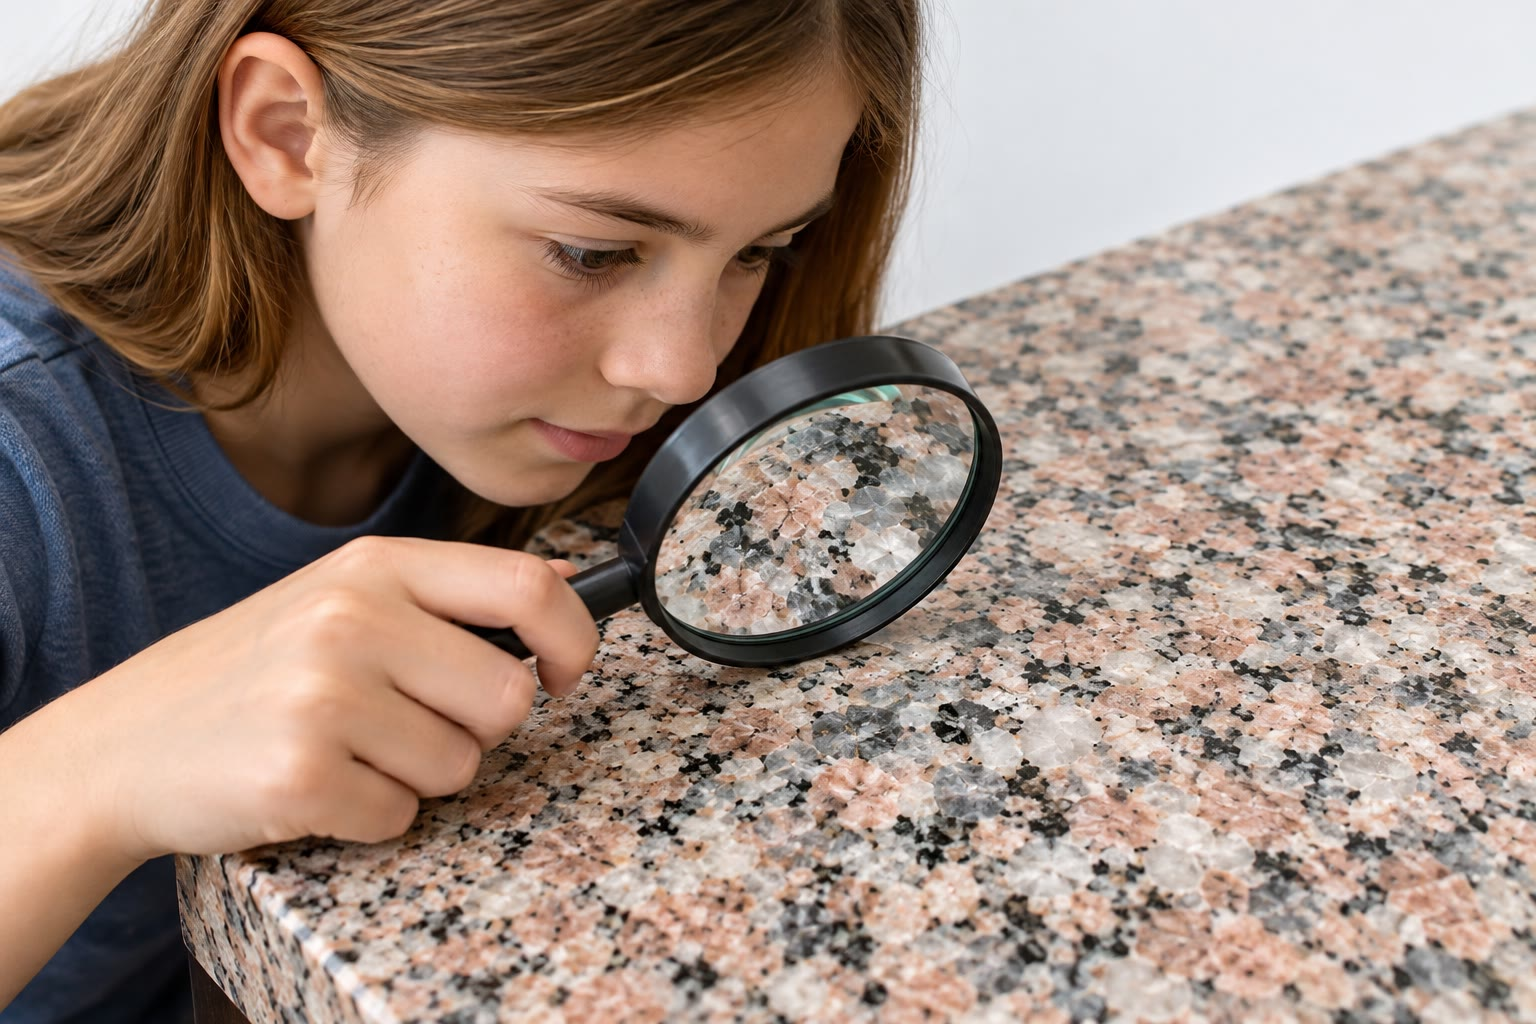
\includegraphics[width=0.6\linewidth]{images/book1/ai/g6-hand-lens-worktop.jpg}

{\small Una encimera de piedra moteada vista con una lupa. (Ilustración
generada por IA.)}
\end{omfigure}

\begin{recall}
Las \omterm{def:g3:stones-pebbles-sand:rock}{rocas} son el material duro de la corteza de la Tierra: pueden romperse
en piedras, los \omterm{def:g1:landscapes-around-us:water}{ríos} las redondean en \omterm{def:g3:stones-pebbles-sand:pebble}{cantos rodados} y se muelen hasta
formar \omterm{def:g3:stones-pebbles-sand:sand}{arena} (\cref{ch:g3:stones-pebbles-sand}). El agua, el hielo y el
viento desgastan las \omterm{def:g3:stones-pebbles-sand:rock}{rocas} (\omterm{def:g5:water-shapes-the-land:weathering}{meteorización}), se llevan los trozos (\omterm{def:g5:water-shapes-the-land:erosion}{erosión})
y los dejan más abajo (\omterm{def:g5:water-shapes-the-land:deposition}{sedimentación}) (\cref{ch:g5:water-shapes-the-land}).
En un \omterm{def:g4:volcanoes-earthquakes-first-look:volcano}{volcán}, la \omterm{def:g3:stones-pebbles-sand:rock}{roca} fundida sale en forma de \omterm{def:g4:volcanoes-earthquakes-first-look:eruption}{lava}
(\cref{ch:g4:volcanoes-earthquakes-first-look}).
\end{recall}

\section{Una roca está hecha de minerales}

Las motas de la encimera son \omterm{def:g6:rocks-and-minerals:mineral}{minerales}, y la piedra es un granito.

\begin{definition}[Mineral]\label{def:g6:rocks-and-minerals:mineral}
Un \emph{mineral}\index{mineral} es una sustancia sólida natural, no
fabricada por los seres vivos, siempre con la misma composición y con sus
átomos ordenados de forma regular. Una \emph{\omterm{def:g3:stones-pebbles-sand:rock}{roca}} está hecha de un solo
mineral o, más a menudo, de varios minerales unidos entre sí.
% ledger: usgs:mineral-rock
\end{definition}

El granito está hecho sobre todo de tres \omterm{def:g6:rocks-and-minerals:mineral}{minerales}: el \emph{feldespato}
(rosa o blanco), el \emph{cuarzo} (gris y vidrioso) y la \emph{mica} (negra
o plateada, en láminas finas y brillantes). Otras \omterm{def:g3:stones-pebbles-sand:rock}{rocas} están hechas de un
solo \omterm{def:g6:rocks-and-minerals:mineral}{mineral}: la caliza, por ejemplo, está hecha casi solo de calcita.
% ledger: nps:granite-minerals, usgs:mineral-rock

\begin{omfigure}
\begin{minipage}[c]{0.5\linewidth}\centering
\begin{tikzpicture}
  \begin{axis}[axis equal image, hide axis, width=\linewidth,
      xmin=0, xmax=6, ymin=0, ymax=4]
    \addplot[fill=orange!35!pink, draw=black!55, line width=0.4pt]
      table {figdata/out/grade-6-granite_mosaic-feldspar.dat};
    \addplot[fill=black!12, draw=black!55, line width=0.4pt]
      table {figdata/out/grade-6-granite_mosaic-quartz.dat};
    \addplot[fill=black!85, draw=black!55, line width=0.4pt]
      table {figdata/out/grade-6-granite_mosaic-mica.dat};
  \end{axis}
\end{tikzpicture}

{\small \tikz\fill[orange!35!pink, draw=black!55] (0,0) rectangle (0.25,0.18); feldespato\quad
\tikz\fill[black!12, draw=black!55] (0,0) rectangle (0.25,0.18); cuarzo\quad
\tikz\fill[black!85] (0,0) rectangle (0.25,0.18); mica}
\end{minipage}\hfill
\begin{minipage}[c]{0.46\linewidth}\centering
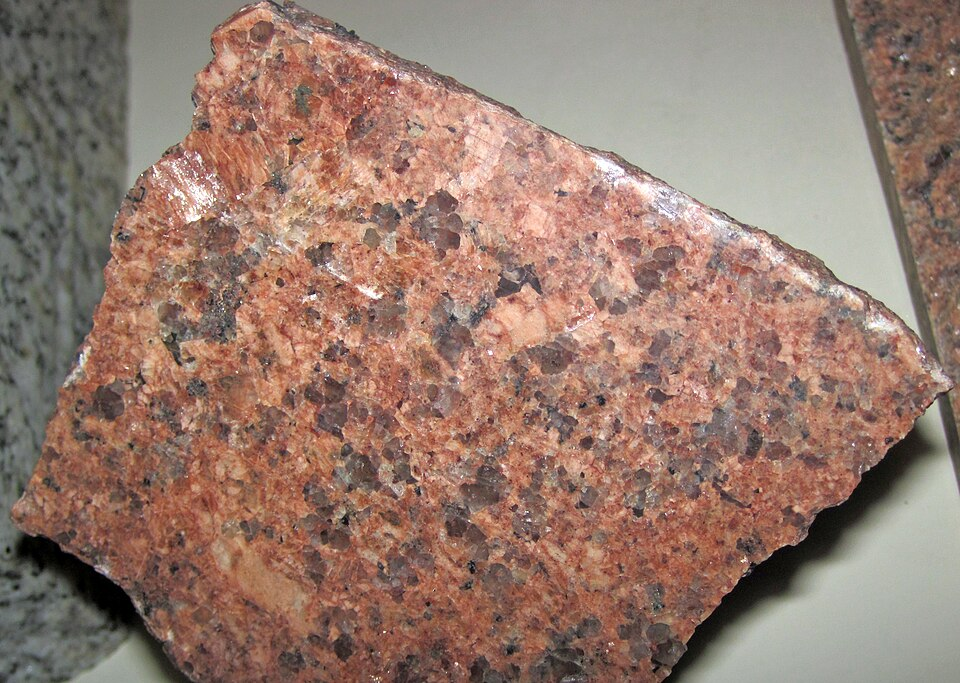
\includegraphics[width=\linewidth]{images/book1/g6-granite.jpg}
\end{minipage}

\smallskip
{\small A la izquierda, el granito dibujado como un mosaico de granos, cada
grano un \omterm{def:g6:rocks-and-minerals:mineral}{mineral} (una ampliación, no a escala). A la derecha, un granito
rosa real, del tamaño de una mano. (Foto: James St.~John, CC BY 2.0, vía
Wikimedia Commons.)}
% ledger: nps:granite-minerals, commons:jsj-rocks (figdata/grade-6/granite_mosaic.py)
\end{omfigure}

\section{Los cristales}

Con la lupa, muchos granos de \omterm{def:g6:rocks-and-minerals:mineral}{mineral} muestran caras planas y brillantes y
aristas rectas. Donde un \omterm{def:g6:rocks-and-minerals:mineral}{mineral} ha tenido sitio para crecer libremente, en
un hueco de la \omterm{def:g3:stones-pebbles-sand:rock}{roca}, forma un cristal: un sólido de forma regular limitado
por caras planas. Su forma se debe a la ordenación regular de sus átomos,
que se estudia en los libros de química. Un cristal de cuarzo, por ejemplo,
es una columna de seis lados que termina en punta; un cristal de mica se
separa en láminas más finas que el papel.

\begin{omfigure}
\begin{minipage}[c]{0.2\linewidth}\centering
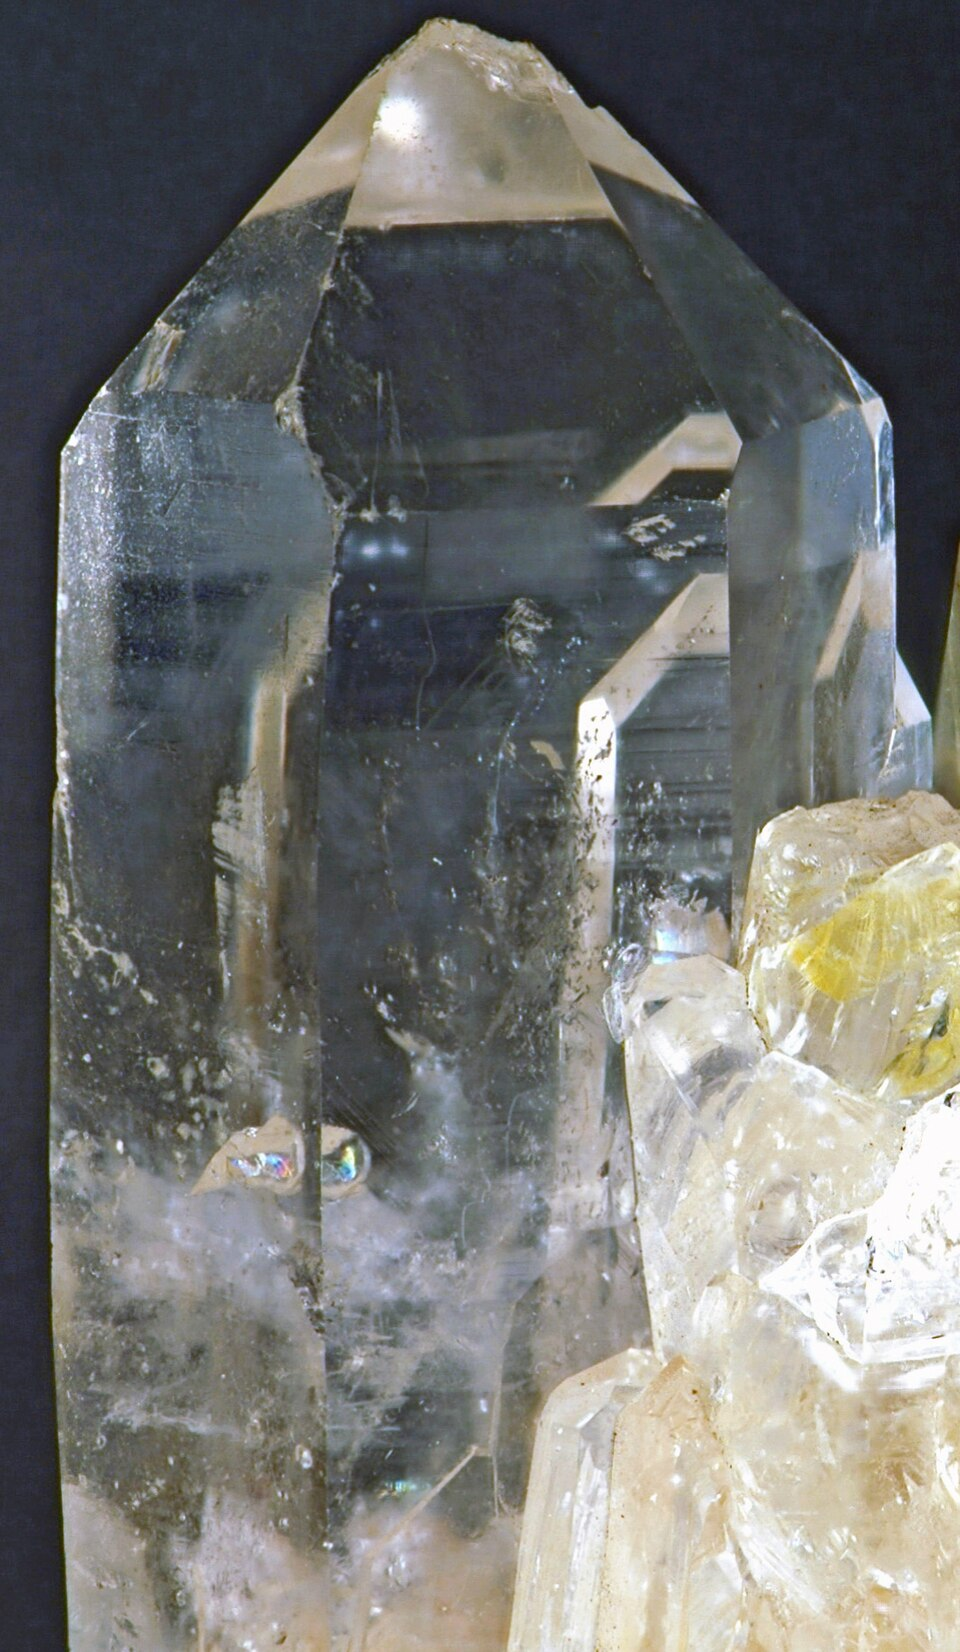
\includegraphics[height=4.2cm]{images/book1/g6-quartz.jpg}
\end{minipage}\hfill
\begin{minipage}[c]{0.44\linewidth}\centering
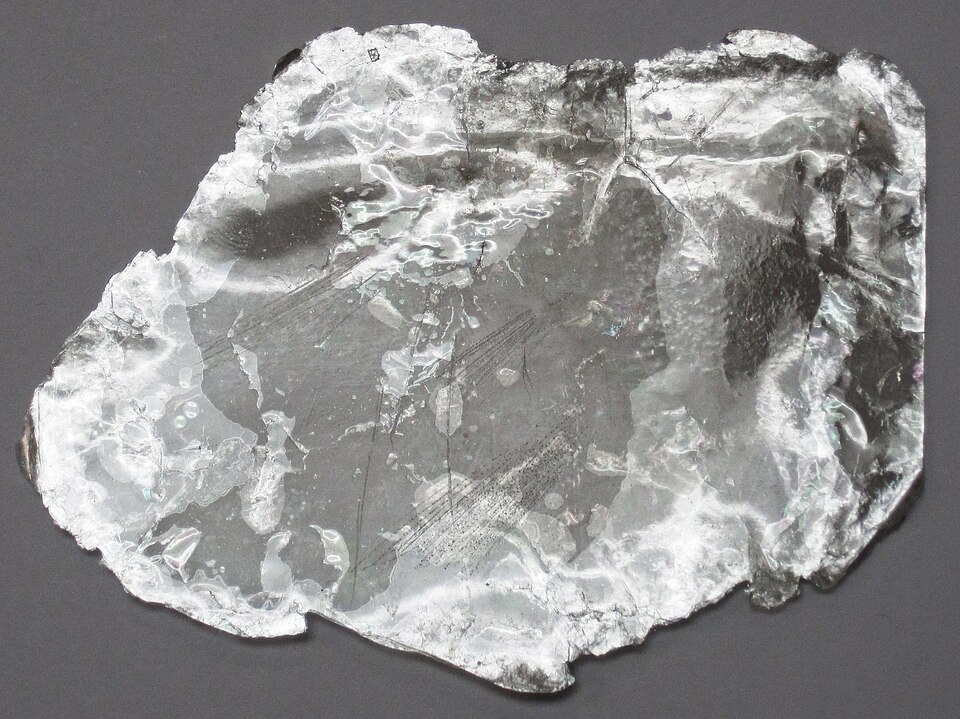
\includegraphics[height=4.2cm]{images/book1/g6-mica.jpg}
\end{minipage}\hfill
\begin{minipage}[c]{0.28\linewidth}
{\small A la izquierda, un cristal de cuarzo, con sus caras planas. A la
derecha, una lámina de mica, un \omterm{def:g6:rocks-and-minerals:mineral}{mineral} que se separa en escamas muy
finas. (Fotos: James St.~John, CC BY 2.0, vía Wikimedia Commons.)}
% ledger: commons:jsj-rocks
\end{minipage}
\end{omfigure}

En el granito, los granos crecieron apretados unos contra otros, así que no
tienen formas bonitas: encajan como un rompecabezas. Su tamaño cuenta una
historia. El granito se forma en las profundidades, donde la \omterm{def:g3:stones-pebbles-sand:rock}{roca} fundida
se enfría muy despacio: sus granos tienen tiempo de crecer lo bastante para
verse a simple vista. La \omterm{def:g3:stones-pebbles-sand:rock}{roca} fundida que se enfría deprisa en la
superficie, en forma de \omterm{def:g4:volcanoes-earthquakes-first-look:eruption}{lava}, da \omterm{def:g3:stones-pebbles-sand:rock}{rocas} con granos demasiado pequeños para
verlos.
% ledger: usgs:mineral-rock

\section{Las tres familias de rocas}

Los geólogos clasifican las \omterm{def:g3:stones-pebbles-sand:rock}{rocas} en tres familias, no por su color, sino
por la manera en que se formaron.

\begin{definition}[Las tres familias de rocas]\label{def:g6:rocks-and-minerals:rock-families}
Una \emph{roca ígnea}\index{roca ignea@roca ígnea} se forma cuando la \omterm{def:g3:stones-pebbles-sand:rock}{roca}
fundida se enfría y se vuelve sólida: el granito en las profundidades, el
basalto a partir de la \omterm{def:g4:volcanoes-earthquakes-first-look:eruption}{lava}.
Una \emph{roca sedimentaria}\index{roca sedimentaria} se forma en la
superficie de la Tierra a partir de granos de \omterm{def:g3:stones-pebbles-sand:sand}{arena} y de \omterm{def:g3:stones-pebbles-sand:sand}{barro}, o de las
conchas de seres vivos, depositados en capas y después endurecidos: la
arenisca, la lutita, la caliza.
Una \emph{roca metamórfica}\index{roca metamorfica@roca metamórfica} es una
\omterm{def:g3:stones-pebbles-sand:rock}{roca} que se ha transformado, sin fundirse, por el calor y la presión en las
profundidades: el mármol (a partir de la caliza), la pizarra (a partir de
la lutita).
% ledger: usgs:mineral-rock, usgs:sedimentary, usgs:metamorphic, geo:marble, geo:slate
\end{definition}

El nombre \emph{ígnea} viene de la palabra latina que significa fuego. Las
\omterm{def:g6:rocks-and-minerals:rock-families}{rocas sedimentarias} muestran a menudo capas, una encima de otra, como las
páginas de un libro. Las \omterm{def:g6:rocks-and-minerals:rock-families}{rocas metamórficas} suelen estar aplastadas y
plegadas; algunas, como la pizarra, se separan en láminas planas.
% ledger: usgs:mineral-rock, usgs:sedimentary, usgs:metamorphic

Muchas \omterm{def:g6:rocks-and-minerals:rock-families}{rocas sedimentarias} están hechas de los granos que clasificaste por
tamaños en el \cref{ch:g3:stones-pebbles-sand}: \omterm{def:g3:stones-pebbles-sand:pebble}{cantos} y \omterm{def:g3:stones-pebbles-sand:pebble}{grava}, \omterm{def:g3:stones-pebbles-sand:sand}{arena},
\omterm{def:g3:stones-pebbles-sand:sand}{barro}. Una vez enterrados, los granos pierden su agua y quedan unidos por un
cemento natural. El tamaño de los granos da nombre a la \omterm{def:g3:stones-pebbles-sand:rock}{roca}.
% ledger: usgs:sedimentary, usgs:wentworth

\begin{omfigure}
\begin{tikzpicture}[
    col/.style={draw=black!60, rounded corners=2pt, minimum width=3.6cm, minimum height=1.9cm},
    lab/.style={font=\scriptsize, align=center}]
  % gravel -> conglomerate
  \node[col, fill=omLithCongl!50] (g) at (0,0) {};
  \foreach \x/\y/\r in {-1.2/0.4/0.32, -0.4/-0.3/0.4, 0.5/0.35/0.3, 1.25/-0.35/0.33, 0.2/-0.55/0.18, -1.3/-0.5/0.22}
    \fill[gray!55, draw=black!60] (\x,\y) circle (\r);
  \node[lab, above=2pt] at (g.north) {\textbf{grava}\\ más de 2~mm};
  \node[lab, below=3pt] (cg) at (g.south) {$\downarrow$ enterrada y cementada\\ \textbf{conglomerado}};
    % sand -> sandstone
  \pgfmathsetseed{7}

  \node[col, fill=omLithSand!60] (s) at (4.2,0) {};
  \foreach \i in {1,...,70} \fill[brown!60!black] ({4.2+1.65*rand},{0.82*rand}) circle (0.045);
  \node[lab, above=2pt] at (s.north) {\textbf{arena}\\ de 2~mm a $\frac{1}{16}$~mm};
  \node[lab, below=3pt] at (s.south) {$\downarrow$ enterrada y cementada\\ \textbf{arenisca}};
  % mud -> shale
  \node[col, fill=omLithShale!70] (m) at (8.4,0) {};
  \foreach \y in {-0.75,-0.5,...,0.8} \draw[black!35, line width=0.3pt] (6.75,\y) -- (10.05,\y);
  \node[lab, above=2pt] at (m.north) {\textbf{barro} (limo y arcilla)\\ menos de $\frac{1}{16}$~mm};
  \node[lab, below=3pt] at (m.south) {$\downarrow$ enterrado y comprimido\\ \textbf{lutita}};
\end{tikzpicture}

{\small Tres \omterm{def:g6:rocks-and-minerals:rock-families}{rocas sedimentarias} que deben su nombre al tamaño de sus
granos (granos muy ampliados; la \omterm{def:g3:stones-pebbles-sand:sand}{arena}, a la escala del recuadro, y la
\omterm{def:g3:stones-pebbles-sand:pebble}{grava}, más grande).}
% ledger: usgs:wentworth, usgs:sedimentary
\end{omfigure}

\begin{inthefield}[Leer las piedras de una ciudad]
Las ciudades son colecciones de \omterm{def:g3:stones-pebbles-sand:rock}{rocas} al aire libre. Pasea con un adulto
junto a muros antiguos, escalinatas, estatuas, fachadas de iglesias y
pavimentos, y míralos de cerca, sin rayar ni romper nada. Algunos bordillos y escalones son de granito: busca su cuarzo vidrioso y su mica brillante. Muchos muros y fachadas antiguos son de caliza o de arenisca: busca conchas, o frota con la yema del dedo una miguita caída de
arenisca para notar la \omterm{def:g3:stones-pebbles-sand:sand}{arena}. Los tejados pueden ser de pizarra, separada
en láminas finas. Apunta en un cuaderno dónde está cada piedra, su color,
sus granos y la familia a la que crees que pertenece; una fotografía ayuda
a compararla después con la tabla de este capítulo.
\end{inthefield}

\section{El ciclo de las rocas}

Las \omterm{def:g3:stones-pebbles-sand:rock}{rocas} no son eternas. Una \omterm{def:g1:landscapes-around-us:landform}{montaña} de granito se meteoriza lentamente;
sus granos son llevados por los \omterm{def:g1:landscapes-around-us:water}{ríos} hasta el \omterm{def:g2:water-on-earth:ocean}{mar} y allí se depositan en
capas; enterradas cada vez más hondo, las capas se endurecen y forman
arenisca. Si la arenisca es llevada todavía más hondo, el calor y la
presión la transforman en una \omterm{def:g6:rocks-and-minerals:rock-families}{roca metamórfica}; más hondo aún, puede
fundirse, y la \omterm{def:g3:stones-pebbles-sand:rock}{roca} fundida, al enfriarse, forma una nueva \omterm{def:g6:rocks-and-minerals:rock-families}{roca ígnea}. Poco
a poco, a lo largo de millones de años, el material de las \omterm{def:g3:stones-pebbles-sand:rock}{rocas} da vueltas
y más vueltas.
% ledger: usgs:sedimentary, usgs:metamorphic

\begin{definition}[Ciclo de las rocas]\label{def:g6:rocks-and-minerals:rock-cycle}
El \emph{ciclo de las rocas}\index{ciclo de las rocas} es el viaje sin fin
por el que las \omterm{def:g3:stones-pebbles-sand:rock}{rocas} de cada familia se transforman lentamente en \omterm{def:g3:stones-pebbles-sand:rock}{rocas} de
las otras familias: por la \omterm{def:g5:water-shapes-the-land:weathering}{meteorización} y la \omterm{def:g5:water-shapes-the-land:erosion}{erosión} en la superficie, por
el enterramiento y el endurecimiento, por el calor y la presión, por la
fusión y el enfriamiento.
\end{definition}

\begin{omfigure}
\begin{tikzpicture}[
    fam/.style={draw, rounded corners=4pt, thick, align=center, minimum width=3.2cm,
                minimum height=1.0cm, font=\small\bfseries},
    stage/.style={draw, dashed, rounded corners=4pt, align=center, minimum width=3.0cm,
                  minimum height=0.9cm, font=\small},
    arr/.style={-{Stealth[length=2.6mm]}, thick},
    lab/.style={font=\scriptsize, align=center, fill=white, inner sep=1.5pt}]
  \node[fam, fill=omLithGranite!60] (ign) at (0,3.6) {rocas ígneas\\[-1pt]{\normalfont\scriptsize granito, basalto}};
  \node[stage, fill=orange!15] (grains) at (6.6,3.6) {granos de arena\\y de barro};
  \node[fam, fill=omLithSand!70] (sed) at (6.6,0) {rocas sedimentarias\\[-1pt]{\normalfont\scriptsize arenisca, lutita, caliza}};
  \node[fam, fill=omLithSchist!60] (met) at (0,0) {rocas metamórficas\\[-1pt]{\normalfont\scriptsize mármol, pizarra}};
  \node[stage, fill=red!12] (melt) at (-4.2,1.8) {roca fundida\\en profundidad};
  \draw[arr] (ign) -- node[lab, above] {meteorización\\y erosión} (grains);
  \draw[arr] (grains) -- node[lab, right] {depositados en capas,\\enterrados, endurecidos} (sed);
  \draw[arr] (sed) -- node[lab, below=2pt] {calor y presión,\\en profundidad} (met);
  \draw[arr] (met) -- node[lab, below left] {fusión} (melt);
  \draw[arr] (melt) -- node[lab, above left] {enfriamiento} (ign);
  \draw[arr, black!55] (met.north east) to[bend left=12] node[lab, pos=0.45, left=4pt, text=black!60] {meteorización} ([xshift=-6pt]grains.south west);
  \draw[arr, black!55] (sed.north west) to[bend left=10] (grains.south west);
\end{tikzpicture}

{\small El \omterm{def:g6:rocks-and-minerals:rock-cycle}{ciclo de las rocas}. Cada flecha tarda desde miles hasta millones
de años. Cualquier \omterm{def:g3:stones-pebbles-sand:rock}{roca} que sale a la superficie puede meteorizarse
(flechas grises).}
% ledger: usgs:sedimentary, usgs:metamorphic, usgs:mineral-rock
\end{omfigure}

\section{Reconocer las rocas más comunes}

Estas son siete \omterm{def:g3:stones-pebbles-sand:rock}{rocas} que se encuentran a menudo en edificios, aceras y
\omterm{def:g1:landscapes-around-us:landscape}{paisajes}.

\begin{omfigure}
\newcommand{\gsixrock}[2]{\begin{minipage}[t]{0.235\linewidth}\centering
  \includegraphics[width=\linewidth, height=0.72\linewidth, keepaspectratio=false]{images/book1/#1}\\[1pt]
  {\footnotesize #2}\end{minipage}}
\gsixrock{g6-granite.jpg}{granito}\hfill
\gsixrock{g6-basalt.jpg}{basalto}\hfill
\gsixrock{g6-sandstone.jpg}{arenisca}\hfill
\gsixrock{g6-limestone.jpg}{caliza (con conchas)}\par\medskip
\gsixrock{g6-shale.jpg}{lutita}\hspace{0.02\linewidth}%
\gsixrock{g6-marble.jpg}{mármol}\hspace{0.02\linewidth}%
\gsixrock{g6-slate-roof.jpg}{pizarra, en un tejado}

\medskip
{\small Siete \omterm{def:g3:stones-pebbles-sand:rock}{rocas} comunes. (Fotos: James St.~John, CC BY 2.0; tejado:
Øyvind Holmstad, CC0; vía Wikimedia Commons.)}
% ledger: commons:jsj-rocks, commons:roof-slates
\end{omfigure}

\begin{center}
\small
\begin{tabular}{>{\raggedright\arraybackslash}p{0.13\linewidth}>{\raggedright\arraybackslash}p{0.15\linewidth}>{\raggedright\arraybackslash}p{0.6\linewidth}}
\hline
\omterm{def:g3:stones-pebbles-sand:rock}{roca} & familia & qué buscar\\
\hline
granito & ígnea & granos grandes de varios colores: feldespato rosa o blanco, cuarzo gris y vidrioso, mica negra y brillante\\
basalto & ígnea & de gris oscuro a negro, granos demasiado pequeños para verlos, a menudo pequeños agujeros redondos dejados por burbujas de gas\\
arenisca & sedimentaria & granos de \omterm{def:g3:stones-pebbles-sand:sand}{arena} que se notan al tacto, áspera como el papel de lija\\
caliza & sedimentaria & clara, a menudo con conchas; burbujea con una gota de ácido diluido\\
lutita & sedimentaria & muy fina y blanda, hecha de \omterm{def:g3:stones-pebbles-sand:sand}{barro} (arcilla) endurecido; en capas finas\\
mármol & metamórfica & blanco o de color, hecho de cristales brillantes que centellean como el azúcar; burbujea con el ácido\\
pizarra & metamórfica & gris, muy fina, se separa en láminas finas, duras y planas\\
\hline
\end{tabular}
% ledger: nps:granite-minerals, geo:basalt, usgs:sedimentary, geo:limestone, geo:marble, geo:slate
\end{center}

\begin{safety}
La prueba del ácido la hace solo un adulto, con gafas y guantes, usando un
ácido muy diluido. No pruebes nunca una \omterm{def:g3:stones-pebbles-sand:rock}{roca} ni un polvo, y no rompas nunca
\omterm{def:g3:stones-pebbles-sand:rock}{rocas} con una herramienta: mirar con una lupa ya dice muchísimo.
% ledger: geo:limestone
\end{safety}

Una clave es una lista de preguntas, cada una con dos respuestas, que lleva
paso a paso hasta el nombre de una \omterm{def:g3:stones-pebbles-sand:rock}{roca}.

\begin{omfigure}
\begin{tikzpicture}[
    q/.style={draw, rounded corners=3pt, fill=omRecall!10, align=center, text width=3.7cm,
              font=\scriptsize, inner sep=3pt},
    r/.style={draw, rounded corners=3pt, thick, fill=omLithSand!40, font=\scriptsize\bfseries,
              align=center, minimum width=1.7cm, inner sep=3pt},
    arr/.style={-{Stealth[length=2mm]}, thick}, yn/.style={font=\scriptsize\itshape, fill=white, inner sep=1pt}]
  \node[q] (q1) at (0,0) {¿Burbujea con una gota de ácido diluido?};
  \node[q] (q2) at (-3.4,-1.6) {¿Se ven conchas, o parece mate y fina?};
  \node[r] (lime) at (-4.8,-3.4) {caliza};
  \node[r, align=center] (marb) at (-2.0,-3.4) {mármol\\[-1pt]{\normalfont\tiny cristales brillantes}};
  \node[q] (q3) at (3.2,-1.6) {¿Se ven granos de varios colores, rosa, gris, negro?};
  \node[r] (gran) at (6.9,-1.6) {granito};
  \node[q] (q4) at (3.2,-3.2) {¿Oscura, con granos invisibles y agujeritos redondos?};
  \node[r] (bas) at (6.9,-3.2) {basalto};
  \node[q] (q5) at (3.2,-4.8) {¿Áspera como el papel de lija, hecha de granos de arena?};
  \node[r] (sand) at (6.9,-4.8) {arenisca};
  \node[q] (q6) at (3.2,-6.4) {¿Dura, se separa en láminas finas y planas?};
  \node[r] (slat) at (6.9,-6.4) {pizarra};
  \node[r] (shal) at (3.2,-7.8) {lutita};
  \draw[arr] (q1) -| node[yn, pos=0.25] {sí} (q2);
  \draw[arr] (q1) -| node[yn, pos=0.25] {no} (q3);
  \draw[arr] (q2.south-|lime) -- node[yn, right] {sí} (lime);
  \draw[arr] (q2.south-|marb) -- node[yn, right] {no} (marb);
  \foreach \a/\b in {q3/gran, q4/bas, q5/sand, q6/slat}{\draw[arr] (\a) -- node[yn, above] {sí} (\b);}
  \foreach \a/\b in {q3/q4, q4/q5, q5/q6, q6/shal}{\draw[arr] (\a) -- node[yn, right] {no} (\b);}
\end{tikzpicture}

{\small Una clave para las siete \omterm{def:g3:stones-pebbles-sand:rock}{rocas} de la tabla. Empieza por arriba y
contesta a cada pregunta con sí o no.}
% ledger: geo:limestone, geo:marble, nps:granite-minerals, geo:basalt, usgs:sedimentary, geo:slate
\end{omfigure}

\paragraph{La dureza.} Hay otra pista que ayuda a reconocer un \omterm{def:g6:rocks-and-minerals:mineral}{mineral}: la
facilidad con que se raya.

\begin{definition}[Dureza y escala de Mohs]\label{def:g6:rocks-and-minerals:hardness}
La \emph{dureza}\index{dureza} de un \omterm{def:g6:rocks-and-minerals:mineral}{mineral} es lo bien que resiste a ser
rayado: un \omterm{def:g6:rocks-and-minerals:mineral}{mineral} raya a todos los más blandos que él y es rayado por
todos los más duros. La \emph{escala de Mohs}\index{escala de Mohs} ordena
la dureza de 1 a 10 con diez \omterm{def:g6:rocks-and-minerals:mineral}{minerales} de referencia, desde el talco (1),
el más blando, hasta el diamante (10), el más duro.
% ledger: nps:mohs-ladder, nps:mohs-testers
\end{definition}

\begin{omfigure}
\begin{tikzpicture}[x=1cm, y=0.62cm]
  \draw[thick, black!60] (0,0.5) -- (0,10.5);
  \foreach \n/\m in {1/talco, 2/yeso, 3/calcita, 4/fluorita, 5/apatito,
                     6/feldespato (ortoclasa), 7/cuarzo, 8/topacio, 9/corindón, 10/diamante}{
    \fill[omRecall!25, draw=black!50] (-0.32,\n-0.32) rectangle (0.32,\n+0.32);
    \node[font=\scriptsize\bfseries] at (0,\n) {\n};
    \node[font=\scriptsize, anchor=east] at (-0.5,\n) {\m};}
  \foreach \v/\t in {2.5/uña, 3.5/moneda de cobre, 5.5/vidrio, 6.5/clavo de acero}{
    \draw[red!70!black, thick] (0.4,\v) -- (1.0,\v);
    \node[font=\scriptsize, red!70!black, anchor=west] at (1.05,\v) {\t\ (unos \v)};}
  \node[font=\scriptsize\itshape, anchor=south] at (0,10.6) {más duro};
  \node[font=\scriptsize\itshape, anchor=north] at (0,0.4) {más blando};
  \node[font=\scriptsize, align=left, anchor=west, text width=6.2cm] at (4.3,5.5)
    {Una uña raya el talco y el yeso, pero no la calcita. Una moneda de
     cobre raya la calcita. El cuarzo raya el vidrio y el acero; ninguno de los cuatro instrumentos de prueba raya el cuarzo. La mica, de 2 a 3, apenas se deja rayar con
     una uña.};
\end{tikzpicture}

{\small La \omterm{def:g6:rocks-and-minerals:hardness}{escala de Mohs} (a la izquierda, los diez \omterm{def:g6:rocks-and-minerals:mineral}{minerales} de referencia)
y cuatro instrumentos de prueba de la vida diaria (a la derecha, en rojo).}
% ledger: nps:mohs-ladder, nps:mohs-testers, geo:mica-hardness
\end{omfigure}

\begin{method}[La prueba del rayado]\label{met:g6:rocks-and-minerals:scratch}
\begin{enumerate}
  \item Intenta rayar el \omterm{def:g6:rocks-and-minerals:mineral}{mineral} con la uña y después con una moneda de
        cobre. (El vidrio y el acero los usa solo un adulto.)
  \item Frota la marca con un dedo: una raya de verdad se queda; un rastro
        de polvo del instrumento de prueba se borra.
  \item La \omterm{def:g6:rocks-and-minerals:hardness}{dureza} está entre la del instrumento más duro que no lo raya y
        la del instrumento más blando que sí lo raya.
\end{enumerate}
\end{method}

\begin{example}[¿Cuarzo o calcita?]\label{ex:g6:rocks-and-minerals:quartz-calcite}
Dos \omterm{def:g6:rocks-and-minerals:mineral}{minerales} blancos se parecen. El primero lo raya una moneda de cobre:
su \omterm{def:g6:rocks-and-minerals:hardness}{dureza} es menor que 3.5; es calcita (3). El segundo no lo raya un clavo
de acero y raya el vidrio: su \omterm{def:g6:rocks-and-minerals:hardness}{dureza} es mayor que 6.5; entre los \omterm{def:g6:rocks-and-minerals:mineral}{minerales}
de referencia, es el cuarzo (7).
% ledger: nps:mohs-ladder, nps:mohs-testers
\end{example}

\section{Ejercicios}

\begin{exercise}[$\star$]\label{exo:g6:rocks-and-minerals:1}
¿A qué familia pertenece cada \omterm{def:g3:stones-pebbles-sand:rock}{roca}: granito, arenisca, mármol, basalto,
caliza, pizarra?
\end{exercise}

\begin{exercise}[$\star$]\label{exo:g6:rocks-and-minerals:2}
¿El cuarzo es un \omterm{def:g6:rocks-and-minerals:mineral}{mineral} o una \omterm{def:g3:stones-pebbles-sand:rock}{roca}? ¿Y el granito? Explica la diferencia
en una frase.
\end{exercise}

\begin{exercise}[$\star$]\label{exo:g6:rocks-and-minerals:3}
Ordena estos \omterm{def:g6:rocks-and-minerals:mineral}{minerales} del más blando al más duro: cuarzo, talco, diamante,
calcita. ¿Cuál de ellos puede rayar a todos los demás?
\end{exercise}

\begin{exercise}[$\star$]\label{exo:g6:rocks-and-minerals:4}
Copia y completa con las palabras \emph{enfriamiento}, \emph{calor y
presión}, \emph{\omterm{def:g5:water-shapes-the-land:weathering}{meteorización}}: ``La \omterm{def:g3:stones-pebbles-sand:rock}{roca} fundida se convierte en una \omterm{def:g6:rocks-and-minerals:rock-families}{roca
ígnea} por \ldots{} Una caliza se convierte en un mármol por \ldots{} Un
granito se convierte en granos de \omterm{def:g3:stones-pebbles-sand:sand}{arena} por \ldots''
\end{exercise}

\begin{exercise}[$\star\star$]\label{exo:g6:rocks-and-minerals:5}
Usa la clave. (a) Una \omterm{def:g3:stones-pebbles-sand:rock}{roca} no burbujea con el ácido; es oscura, con granos
demasiado pequeños para verlos y pequeños agujeros redondos. (b) Una \omterm{def:g3:stones-pebbles-sand:rock}{roca}
burbujea con el ácido y está hecha de cristales brillantes que centellean
como el azúcar. (c) Una \omterm{def:g3:stones-pebbles-sand:rock}{roca} no burbujea; es áspera como el papel de lija.
Di el nombre de cada \omterm{def:g3:stones-pebbles-sand:rock}{roca}.
\end{exercise}

\begin{exercise}[$\star\star$]\label{exo:g6:rocks-and-minerals:6}
Un \omterm{def:g6:rocks-and-minerals:mineral}{mineral} se raya con una moneda de cobre, pero no con la uña. ¿Entre qué
dos valores de \omterm{def:g6:rocks-and-minerals:hardness}{dureza} está? ¿Qué \omterm{def:g6:rocks-and-minerals:mineral}{mineral} de referencia de la \omterm{def:g6:rocks-and-minerals:hardness}{escala de Mohs}
podría ser?
\end{exercise}

\begin{exercise}[$\star\star$]\label{exo:g6:rocks-and-minerals:7}
% exercise data: figdata/grade-6/granite_mosaic.py (33 / 21 / 6 grains)
En el dibujo del granito de este capítulo hay 60 granos: 33 de feldespato,
21 de cuarzo y 6 de mica. ¿Qué porcentaje de los granos es de cuarzo? ¿Y de
feldespato? ¿Y de mica? Comprueba que los tres porcentajes suman
100~\%.
\end{exercise}

\begin{exercise}[$\star\star$]\label{exo:g6:rocks-and-minerals:8}
El granito y el basalto son, los dos, \omterm{def:g6:rocks-and-minerals:rock-families}{rocas ígneas}. ¿Por qué vemos a simple
vista los granos del granito, pero no los del basalto?
\end{exercise}

\begin{exercise}[$\star\star$]\label{exo:g6:rocks-and-minerals:9}
El mármol se forma a partir de la caliza. (a) ¿A qué familia pertenece cada
una? (b) ¿Qué le pasó a la caliza para convertirse en mármol? (c) ¿Por qué
burbujean las dos con el ácido?
\end{exercise}

\begin{exercise}[$\star\star$]\label{exo:g6:rocks-and-minerals:10}
Usa la \omterm{def:g6:rocks-and-minerals:hardness}{escala de Mohs}: (a) ¿puede el cuarzo rayar una botella de vidrio?
(b) ¿Y la fluorita? (c) ¿Puede un clavo de acero rayar el feldespato?
\end{exercise}

\begin{exercise}[$\star\star\star$]\label{exo:g6:rocks-and-minerals:11}
Cuenta en cinco etapas el viaje de un grano de cuarzo, desde una \omterm{def:g1:landscapes-around-us:landform}{montaña} de
granito hasta una \omterm{def:g6:rocks-and-minerals:rock-families}{roca metamórfica}. Di el nombre del proceso en cada etapa
y la familia de la \omterm{def:g3:stones-pebbles-sand:rock}{roca} al principio y al final.
\end{exercise}

\begin{exercise}[$\star\star\star$]\label{exo:g6:rocks-and-minerals:12}
Un \omterm{def:g6:rocks-and-minerals:mineral}{mineral} gris y vidrioso no se raya con un clavo de acero, raya el
vidrio y es rayado por el topacio. (a) ¿Cuál es su \omterm{def:g6:rocks-and-minerals:hardness}{dureza} en la \omterm{def:g6:rocks-and-minerals:hardness}{escala de
Mohs}? Di su nombre. (b) Los granos de \omterm{def:g3:stones-pebbles-sand:sand}{arena} ruedan durante años empujados
por las olas y los \omterm{def:g1:landscapes-around-us:water}{ríos}. Usa su \omterm{def:g6:rocks-and-minerals:hardness}{dureza} para explicar por qué los granos de
este \omterm{def:g6:rocks-and-minerals:mineral}{mineral} duran mucho más que los de calcita o de mica.
\end{exercise}

\section{Problema: las piedras de la plaza del pueblo}

\begin{problem}[{Problema de fin de semana --- las rocas de una plaza, el
mineral más duro de todos y cuántas familias de rocas hay}]
\label{pb:g6:rocks-and-minerals:1}
% ledger: nps:granite-minerals, geo:limestone, geo:slate, geo:marble, nps:mohs-ladder, nps:mohs-testers, geo:mica-hardness
En una excursión escolar, la clase observa las piedras de la vieja plaza
del pueblo (solo se observa: nadie rompe ni raya los monumentos). La
maestra ha traído del taller del cantero trozos sueltos de las mismas
piedras para las pruebas de \omterm{def:g6:rocks-and-minerals:hardness}{dureza}.

\smallskip
\noindent\textbf{La fuente}: su pilón muestra granos grandes, rosas,
        blancos, grises y vidriosos, y negros y brillantes.
\textbf{El pavimento}: losas claras en las que se ven pequeñas conchas
        fósiles; una gota de ácido diluido, que pone la maestra sobre un
        trozo suelto, burbujea.
\textbf{El tejado del ayuntamiento}: láminas finas, planas y grises de una
        piedra de grano muy fino.
\textbf{La estatua}: una piedra blanca hecha de cristales brillantes que
        centellean como el azúcar; también burbujea.

\medskip
\noindent\textbf{Parte I --- La fuente, el pavimento, el tejado.}
\begin{enumerate}
  \item Di el nombre de la \omterm{def:g3:stones-pebbles-sand:rock}{roca} de la fuente y su familia. Nombra sus tres
        \omterm{def:g6:rocks-and-minerals:mineral}{minerales}.
  \item Di el nombre de la \omterm{def:g3:stones-pebbles-sand:rock}{roca} del pavimento y su familia. ¿Qué eran las
        conchas antes de estar en la piedra?
  \item Di el nombre de la \omterm{def:g3:stones-pebbles-sand:rock}{roca} del tejado y su familia. ¿A partir de qué
        \omterm{def:g3:stones-pebbles-sand:rock}{roca} se formó?
  \item Di el nombre de la \omterm{def:g3:stones-pebbles-sand:rock}{roca} de la estatua y su familia. ¿A partir de
        qué \omterm{def:g3:stones-pebbles-sand:rock}{roca} se formó?
\end{enumerate}

\medskip
\noindent\textbf{Parte II --- Una prueba de dureza.}
\begin{enumerate}[resume]
  \item La maestra intenta rayar con un clavo de acero un grano gris y
        vidrioso de la fuente: no hay raya. El grano raya el vidrio. ¿Qué
        \omterm{def:g6:rocks-and-minerals:mineral}{mineral} es y cuál es su \omterm{def:g6:rocks-and-minerals:hardness}{dureza}?
  \item Los granos rosas se rayan con el clavo de acero, pero no con el
        vidrio. ¿Entre qué dos valores está su \omterm{def:g6:rocks-and-minerals:hardness}{dureza}? ¿Qué \omterm{def:g6:rocks-and-minerals:mineral}{mineral} de la
        \omterm{def:g6:rocks-and-minerals:hardness}{escala de Mohs} es?
  \item Las escamas negras apenas se dejan rayar con la uña. ¿Qué \omterm{def:g6:rocks-and-minerals:mineral}{mineral}
        es?
  \item ¿Puede una moneda de cobre rayar el pavimento? Explícalo con la
        \omterm{def:g6:rocks-and-minerals:hardness}{dureza} de la calcita.
\end{enumerate}

\medskip
\noindent\textbf{Parte III --- El ciclo de las rocas.}
\begin{enumerate}[resume]
  \item Después de siglos de \omterm{def:g4:clouds-rain-snow:precipitation}{lluvia}, la estatua ha perdido sus detalles
        finos. ¿Qué proceso del \omterm{def:g6:rocks-and-minerals:rock-cycle}{ciclo de las rocas} está actuando?
  \item El granito de la fuente vino de una \omterm{def:g1:landscapes-around-us:landform}{montaña}. A lo largo de
        millones de años, ¿en qué podrían convertirse los granos de cuarzo
        de esa \omterm{def:g1:landscapes-around-us:landform}{montaña}, y en qué \omterm{def:g3:stones-pebbles-sand:rock}{roca} podrían acabar?
  \item ¿Cuántas de las tres familias de \omterm{def:g3:stones-pebbles-sand:rock}{rocas} hay en la plaza? Di el
        nombre de la \omterm{def:g3:stones-pebbles-sand:rock}{roca} o de las \omterm{def:g3:stones-pebbles-sand:rock}{rocas} de cada una.
  \item ¿Cuál es la \omterm{def:g6:rocks-and-minerals:hardness}{dureza} de Mohs del \omterm{def:g6:rocks-and-minerals:mineral}{mineral} más duro que hay en las
        piedras de la plaza?
\end{enumerate}
\end{problem}
